% fila 1
La familia de Elena compra 18 aguacates en el mercado agrícola. Hay 3 aguacates en cada bolsa. 
& \node {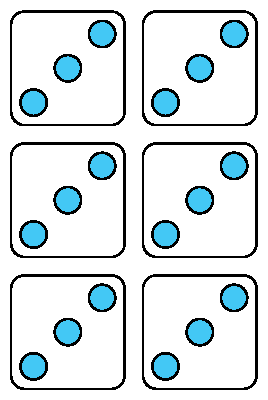
\includegraphics[scale=\figScale]{tikz-file-3-4-B-131870.pdf}};
&    
&  $18 \div 3 = \underline{\hspace{0.7 cm}}$
\\% 
% fila 2
Andre ve 25 tomates. Están en 5 racimos. Cada racimo tiene el mismo número de tomates. 
&  
& $5 \times {?} = 25$ 
& $25 \div 5 = {?}$ 
\\% 
% fila 3
Lin pide 6 buñuelos de banano. Los buñuelos se sirven en 2 platos y cada plato tiene el mismo número de buñuelos. 
& \node {
\includegraphics[scale=\figScale]{tikz-file-3-4-B-131871.pdf}};
& $2 \times{ ?} = 6$ 
&   
\\%
% fila 4
% 
& \node {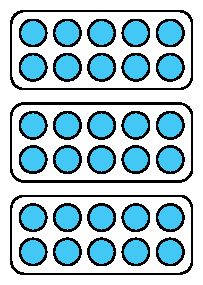
\includegraphics[scale=\figScale]{tikz-file-3-4-B-131872.pdf}};
& $\underline{\hspace{0.7 cm}} \times 10 = 30$ 
&  $30 \div 10 = \underline{\hspace{0.7 cm}}$ 